\documentclass[1p]{elsarticle_modified}
%\bibliographystyle{elsarticle-num}

%\usepackage[colorlinks]{hyperref}
%\usepackage{abbrmath_seonhwa} %\Abb, \Ascr, \Acal ,\Abf, \Afrak
\usepackage{amsfonts}
\usepackage{amssymb}
\usepackage{amsmath}
\usepackage{amsthm}
\usepackage{scalefnt}
\usepackage{amsbsy}
\usepackage{kotex}
\usepackage{caption}
\usepackage{subfig}
\usepackage{color}
\usepackage{graphicx}
\usepackage{xcolor} %% white, black, red, green, blue, cyan, magenta, yellow
\usepackage{float}
\usepackage{setspace}
\usepackage{hyperref}

\usepackage{tikz}
\usetikzlibrary{arrows}

\usepackage{multirow}
\usepackage{array} % fixed length table
\usepackage{hhline}

%%%%%%%%%%%%%%%%%%%%%
\makeatletter
\renewcommand*\env@matrix[1][\arraystretch]{%
	\edef\arraystretch{#1}%
	\hskip -\arraycolsep
	\let\@ifnextchar\new@ifnextchar
	\array{*\c@MaxMatrixCols c}}
\makeatother %https://tex.stackexchange.com/questions/14071/how-can-i-increase-the-line-spacing-in-a-matrix
%%%%%%%%%%%%%%%

\usepackage[normalem]{ulem}

\newcommand{\msout}[1]{\ifmmode\text{\sout{\ensuremath{#1}}}\else\sout{#1}\fi}
%SOURCE: \msout is \stkout macro in https://tex.stackexchange.com/questions/20609/strikeout-in-math-mode

\newcommand{\cancel}[1]{
	\ifmmode
	{\color{red}\msout{#1}}
	\else
	{\color{red}\sout{#1}}
	\fi
}

\newcommand{\add}[1]{
	{\color{blue}\uwave{#1}}
}

\newcommand{\replace}[2]{
	\ifmmode
	{\color{red}\msout{#1}}{\color{blue}\uwave{#2}}
	\else
	{\color{red}\sout{#1}}{\color{blue}\uwave{#2}}
	\fi
}

\newcommand{\Sol}{\mathcal{S}} %segment
\newcommand{\D}{D} %diagram
\newcommand{\A}{\mathcal{A}} %arc


%%%%%%%%%%%%%%%%%%%%%%%%%%%%%5 test

\def\sl{\operatorname{\textup{SL}}(2,\Cbb)}
\def\psl{\operatorname{\textup{PSL}}(2,\Cbb)}
\def\quan{\mkern 1mu \triangleright \mkern 1mu}

\theoremstyle{definition}
\newtheorem{thm}{Theorem}[section]
\newtheorem{prop}[thm]{Proposition}
\newtheorem{lem}[thm]{Lemma}
\newtheorem{ques}[thm]{Question}
\newtheorem{cor}[thm]{Corollary}
\newtheorem{defn}[thm]{Definition}
\newtheorem{exam}[thm]{Example}
\newtheorem{rmk}[thm]{Remark}
\newtheorem{alg}[thm]{Algorithm}

\newcommand{\I}{\sqrt{-1}}
\begin{document}

%\begin{frontmatter}
%
%\title{Boundary parabolic representations of knots up to 8 crossings}
%
%%% Group authors per affiliation:
%\author{Yunhi Cho} 
%\address{Department of Mathematics, University of Seoul, Seoul, Korea}
%\ead{yhcho@uos.ac.kr}
%
%
%\author{Seonhwa Kim} %\fnref{s_kim}}
%\address{Center for Geometry and Physics, Institute for Basic Science, Pohang, 37673, Korea}
%\ead{ryeona17@ibs.re.kr}
%
%\author{Hyuk Kim}
%\address{Department of Mathematical Sciences, Seoul National University, Seoul 08826, Korea}
%\ead{hyukkim@snu.ac.kr}
%
%\author{Seokbeom Yoon}
%\address{Department of Mathematical Sciences, Seoul National University, Seoul, 08826,  Korea}
%\ead{sbyoon15@snu.ac.kr}
%
%\begin{abstract}
%We find all boundary parabolic representation of knots up to 8 crossings.
%
%\end{abstract}
%\begin{keyword}
%    \MSC[2010] 57M25 
%\end{keyword}
%
%\end{frontmatter}

%\linenumbers
%\tableofcontents
%
\newcommand\colored[1]{\textcolor{white}{\rule[-0.35ex]{0.8em}{1.4ex}}\kern-0.8em\color{red} #1}%
%\newcommand\colored[1]{\textcolor{white}{ #1}\kern-2.17ex	\textcolor{white}{ #1}\kern-1.81ex	\textcolor{white}{ #1}\kern-2.15ex\color{red}#1	}

{\Large $\underline{12n_{0245}~(K12n_{0245})}$}

\setlength{\tabcolsep}{10pt}
\renewcommand{\arraystretch}{1.6}
\vspace{1cm}\begin{tabular}{m{100pt}>{\centering\arraybackslash}m{274pt}}
\multirow{5}{120pt}{
	\centering
	\includegraphics[width=112pt]{../../../GIT/diagram.site/Diagrams/png/2334_12n_0245.png}\\
\ \ \ A knot diagram\footnotemark}&
\allowdisplaybreaks
\textbf{Linearized knot diagam} \\
\cline{2-2}
 &
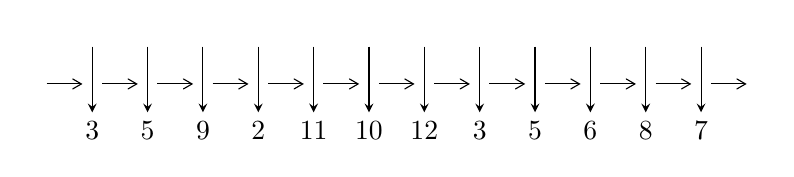
\begin{tikzpicture}[x=20pt, y=17pt]
	% nodes
	\node (C0) at (0, 0) {};
	\node (C1) at (1, 0) {};
	\node (C1U) at (1, +1) {};
	\node (C1D) at (1, -1) {3};

	\node (C2) at (2, 0) {};
	\node (C2U) at (2, +1) {};
	\node (C2D) at (2, -1) {5};

	\node (C3) at (3, 0) {};
	\node (C3U) at (3, +1) {};
	\node (C3D) at (3, -1) {9};

	\node (C4) at (4, 0) {};
	\node (C4U) at (4, +1) {};
	\node (C4D) at (4, -1) {2};

	\node (C5) at (5, 0) {};
	\node (C5U) at (5, +1) {};
	\node (C5D) at (5, -1) {11};

	\node (C6) at (6, 0) {};
	\node (C6U) at (6, +1) {};
	\node (C6D) at (6, -1) {10};

	\node (C7) at (7, 0) {};
	\node (C7U) at (7, +1) {};
	\node (C7D) at (7, -1) {12};

	\node (C8) at (8, 0) {};
	\node (C8U) at (8, +1) {};
	\node (C8D) at (8, -1) {3};

	\node (C9) at (9, 0) {};
	\node (C9U) at (9, +1) {};
	\node (C9D) at (9, -1) {5};

	\node (C10) at (10, 0) {};
	\node (C10U) at (10, +1) {};
	\node (C10D) at (10, -1) {6};

	\node (C11) at (11, 0) {};
	\node (C11U) at (11, +1) {};
	\node (C11D) at (11, -1) {8};

	\node (C12) at (12, 0) {};
	\node (C12U) at (12, +1) {};
	\node (C12D) at (12, -1) {7};
	\node (C13) at (13, 0) {};

	% arrows
	\draw[->,>={angle 60}]
	(C0) edge (C1) (C1) edge (C2) (C2) edge (C3) (C3) edge (C4) (C4) edge (C5) (C5) edge (C6) (C6) edge (C7) (C7) edge (C8) (C8) edge (C9) (C9) edge (C10) (C10) edge (C11) (C11) edge (C12) (C12) edge (C13) ;	\draw[->,>=stealth]
	(C1U) edge (C1D) (C2U) edge (C2D) (C3U) edge (C3D) (C4U) edge (C4D) (C5U) edge (C5D) (C6U) edge (C6D) (C7U) edge (C7D) (C8U) edge (C8D) (C9U) edge (C9D) (C10U) edge (C10D) (C11U) edge (C11D) (C12U) edge (C12D) ;
	\end{tikzpicture} \\
\hhline{~~} \\& 
\textbf{Solving Sequence} \\ \cline{2-2} 
 &
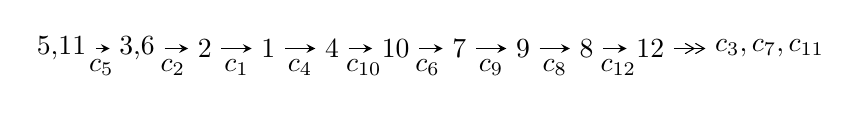
\begin{tikzpicture}[x=23pt, y=7pt]
	% node
	\node (A0) at (-1/8, 0) {5,11};
	\node (A1) at (17/16, 0) {3,6};
	\node (A2) at (17/8, 0) {2};
	\node (A3) at (25/8, 0) {1};
	\node (A4) at (33/8, 0) {4};
	\node (A5) at (41/8, 0) {10};
	\node (A6) at (49/8, 0) {7};
	\node (A7) at (57/8, 0) {9};
	\node (A8) at (65/8, 0) {8};
	\node (A9) at (73/8, 0) {12};
	\node (C1) at (1/2, -1) {$c_{5}$};
	\node (C2) at (13/8, -1) {$c_{2}$};
	\node (C3) at (21/8, -1) {$c_{1}$};
	\node (C4) at (29/8, -1) {$c_{4}$};
	\node (C5) at (37/8, -1) {$c_{10}$};
	\node (C6) at (45/8, -1) {$c_{6}$};
	\node (C7) at (53/8, -1) {$c_{9}$};
	\node (C8) at (61/8, -1) {$c_{8}$};
	\node (C9) at (69/8, -1) {$c_{12}$};
	\node (A10) at (11, 0) {$c_{3},c_{7},c_{11}$};

	% edge
	\draw[->,>=stealth]	
	(A0) edge (A1) (A1) edge (A2) (A2) edge (A3) (A3) edge (A4) (A4) edge (A5) (A5) edge (A6) (A6) edge (A7) (A7) edge (A8) (A8) edge (A9) ;
	\draw[->>,>={angle 60}]	
	(A9) edge (A10);
\end{tikzpicture} \\ 

\end{tabular} \\

\footnotetext{
The image of knot diagram is generated by the software ``\textbf{Draw programme}" developed by Andrew Bartholomew(\url{http://www.layer8.co.uk/maths/draw/index.htm\#Running-draw}), where we modified some parts for our purpose(\url{https://github.com/CATsTAILs/LinksPainter}).
}\phantom \\ \newline 
\centering \textbf{Ideals for irreducible components\footnotemark of $X_{\text{par}}$} 
 
\begin{align*}
I^u_{1}&=\langle 
u^9- u^8+5 u^7-7 u^6+9 u^5-16 u^4+7 u^3-10 u^2+4 b+3 u+3,\\
\phantom{I^u_{1}}&\phantom{= \langle  }u^9+3 u^8+5 u^7+5 u^6+5 u^5-8 u^4-5 u^3-22 u^2+8 a- u-5,\\
\phantom{I^u_{1}}&\phantom{= \langle  }u^{10}+4 u^8-2 u^7+6 u^6-7 u^5+3 u^4-7 u^3+u^2-2 u-1\rangle \\
I^u_{2}&=\langle 
22 u^{15}+71 u^{14}+\cdots+125 b+158,\;121 u^{15}+203 u^{14}+\cdots+125 a-6,\;u^{16}+2 u^{15}+\cdots+2 u+1\rangle \\
I^u_{3}&=\langle 
b+1,\;u^2+2 a+u+3,\;u^3+2 u-1\rangle \\
I^u_{4}&=\langle 
b+1,\;u^3+u^2+a+u+2,\;u^4+u^3+2 u^2+2 u+1\rangle \\
\\
\end{align*}
\raggedright * 4 irreducible components of $\dim_{\mathbb{C}}=0$, with total 33 representations.\\
\footnotetext{All coefficients of polynomials are rational numbers. But the coefficients are sometimes approximated in decimal forms when there is not enough margin.}
\newpage
\renewcommand{\arraystretch}{1}
\centering \section*{I. $I^u_{1}= \langle u^9- u^8+\cdots+4 b+3,\;u^9+3 u^8+\cdots+8 a-5,\;u^{10}+4 u^8+\cdots-2 u-1 \rangle$}
\flushleft \textbf{(i) Arc colorings}\\
\begin{tabular}{m{7pt} m{180pt} m{7pt} m{180pt} }
\flushright $a_{5}=$&$\begin{pmatrix}1\\0\end{pmatrix}$ \\
\flushright $a_{11}=$&$\begin{pmatrix}0\\u\end{pmatrix}$ \\
\flushright $a_{3}=$&$\begin{pmatrix}-\frac{1}{8} u^9-\frac{3}{8} u^8+\cdots+\frac{1}{8} u+\frac{5}{8}\\-\frac{1}{4} u^9+\frac{1}{4} u^8+\cdots-\frac{3}{4} u-\frac{3}{4}\end{pmatrix}$ \\
\flushright $a_{6}=$&$\begin{pmatrix}1\\u^2\end{pmatrix}$ \\
\flushright $a_{2}=$&$\begin{pmatrix}-\frac{3}{8} u^9-\frac{1}{8} u^8+\cdots-\frac{5}{8} u-\frac{1}{8}\\-\frac{1}{4} u^9+\frac{1}{4} u^8+\cdots-\frac{3}{4} u-\frac{3}{4}\end{pmatrix}$ \\
\flushright $a_{1}=$&$\begin{pmatrix}- u^3-2 u\\u^9+3 u^7-2 u^6+2 u^5-5 u^4-3 u^3-2 u^2\end{pmatrix}$ \\
\flushright $a_{4}=$&$\begin{pmatrix}-\frac{13}{8} u^9+\frac{1}{8} u^8+\cdots-\frac{3}{8} u+\frac{1}{8}\\-\frac{5}{4} u^9+\frac{1}{4} u^8+\cdots-\frac{3}{4} u-\frac{3}{4}\end{pmatrix}$ \\
\flushright $a_{10}=$&$\begin{pmatrix}u\\u^3+u\end{pmatrix}$ \\
\flushright $a_{7}=$&$\begin{pmatrix}u^2+1\\u^4+2 u^2\end{pmatrix}$ \\
\flushright $a_{9}=$&$\begin{pmatrix}u^3+2 u\\u^3+u\end{pmatrix}$ \\
\flushright $a_{8}=$&$\begin{pmatrix}-1\\u^8+3 u^6-2 u^5+3 u^4-5 u^3- u^2-2 u-1\end{pmatrix}$ \\
\flushright $a_{12}=$&$\begin{pmatrix}- u\\u^9+3 u^7-2 u^6+3 u^5-5 u^4- u^3-2 u^2\end{pmatrix}$\\&\end{tabular}
\flushleft \textbf{(ii) Obstruction class $= -1$}\\~\\
\flushleft \textbf{(iii) Cusp Shapes $= \frac{15}{16} u^9-\frac{51}{16} u^8+\frac{51}{16} u^7-\frac{197}{16} u^6+\frac{171}{16} u^5-\frac{35}{2} u^4+\frac{293}{16} u^3-\frac{53}{8} u^2+\frac{145}{16} u-\frac{219}{16}$}\\~\\
\newpage\renewcommand{\arraystretch}{1}
\flushleft \textbf{(iv) u-Polynomials at the component}\newline \\
\begin{tabular}{m{50pt}|m{274pt}}
Crossings & \hspace{64pt}u-Polynomials at each crossing \\
\hline $$\begin{aligned}c_{1}\end{aligned}$$&$\begin{aligned}
&u^{10}+14 u^9+\cdots+625 u+16
\end{aligned}$\\
\hline $$\begin{aligned}c_{2},c_{4}\end{aligned}$$&$\begin{aligned}
&u^{10}-2 u^9-5 u^8+7 u^7+14 u^6-36 u^4-8 u^3+42 u^2-17 u-4
\end{aligned}$\\
\hline $$\begin{aligned}c_{3},c_{8}\end{aligned}$$&$\begin{aligned}
&u^{10}+3 u^9+\cdots+88 u+32
\end{aligned}$\\
\hline $$\begin{aligned}c_{5},c_{6},c_{7}\\c_{10},c_{11},c_{12}\end{aligned}$$&$\begin{aligned}
&u^{10}+4 u^8-2 u^7+6 u^6-7 u^5+3 u^4-7 u^3+u^2-2 u-1
\end{aligned}$\\
\hline $$\begin{aligned}c_{9}\end{aligned}$$&$\begin{aligned}
&u^{10}-6 u^9+9 u^8+2 u^7+7 u^6-51 u^5+50 u^4-20 u^3+7 u^2-4 u-4
\end{aligned}$\\
\hline
\end{tabular}\\~\\
\newpage\renewcommand{\arraystretch}{1}
\flushleft \textbf{(v) Riley Polynomials at the component}\newline \\
\begin{tabular}{m{50pt}|m{274pt}}
Crossings & \hspace{64pt}Riley Polynomials at each crossing \\
\hline $$\begin{aligned}c_{1}\end{aligned}$$&$\begin{aligned}
&y^{10}-34 y^9+\cdots-333665 y+256
\end{aligned}$\\
\hline $$\begin{aligned}c_{2},c_{4}\end{aligned}$$&$\begin{aligned}
&y^{10}-14 y^9+\cdots-625 y+16
\end{aligned}$\\
\hline $$\begin{aligned}c_{3},c_{8}\end{aligned}$$&$\begin{aligned}
&y^{10}-15 y^9+\cdots-3392 y+1024
\end{aligned}$\\
\hline $$\begin{aligned}c_{5},c_{6},c_{7}\\c_{10},c_{11},c_{12}\end{aligned}$$&$\begin{aligned}
&y^{10}+8 y^9+\cdots-6 y+1
\end{aligned}$\\
\hline $$\begin{aligned}c_{9}\end{aligned}$$&$\begin{aligned}
&y^{10}-18 y^9+\cdots-72 y+16
\end{aligned}$\\
\hline
\end{tabular}\\~\\
\newpage\flushleft \textbf{(vi) Complex Volumes and Cusp Shapes}
$$\begin{array}{c|c|c}  
\text{Solutions to }I^u_{1}& \I (\text{vol} + \sqrt{-1}CS) & \text{Cusp shape}\\
 \hline 
\begin{aligned}
u &= -0.408860 + 1.019830 I \\
a &= -0.623231 - 0.763538 I \\
b &= -0.84308 + 1.25661 I\end{aligned}
 & \phantom{-}0.76752 + 5.23818 I & -10.88397 - 7.30305 I \\ \hline\begin{aligned}
u &= -0.408860 - 1.019830 I \\
a &= -0.623231 + 0.763538 I \\
b &= -0.84308 - 1.25661 I\end{aligned}
 & \phantom{-}0.76752 - 5.23818 I & -10.88397 + 7.30305 I \\ \hline\begin{aligned}
u &= \phantom{-}1.10481\phantom{ +0.000000I} \\
a &= \phantom{-}1.89244\phantom{ +0.000000I} \\
b &= \phantom{-}1.98176\phantom{ +0.000000I}\end{aligned}
 & -16.4276\phantom{ +0.000000I} & -16.3110\phantom{ +0.000000I} \\ \hline\begin{aligned}
u &= \phantom{-}0.331850 + 0.653227 I \\
a &= -0.698518 + 0.937685 I \\
b &= -1.56733 - 0.09555 I\end{aligned}
 & -1.76206 - 1.44138 I & -14.1408 + 4.6887 I \\ \hline\begin{aligned}
u &= \phantom{-}0.331850 - 0.653227 I \\
a &= -0.698518 - 0.937685 I \\
b &= -1.56733 + 0.09555 I\end{aligned}
 & -1.76206 + 1.44138 I & -14.1408 - 4.6887 I \\ \hline\begin{aligned}
u &= \phantom{-}0.24366 + 1.40906 I \\
a &= \phantom{-}0.325341 - 0.085189 I \\
b &= \phantom{-}0.683278 - 0.384377 I\end{aligned}
 & \phantom{-}8.38588 - 4.49014 I & -3.00164 + 0.77612 I \\ \hline\begin{aligned}
u &= \phantom{-}0.24366 - 1.40906 I \\
a &= \phantom{-}0.325341 + 0.085189 I \\
b &= \phantom{-}0.683278 + 0.384377 I\end{aligned}
 & \phantom{-}8.38588 + 4.49014 I & -3.00164 - 0.77612 I \\ \hline\begin{aligned}
u &= -0.56211 + 1.36382 I \\
a &= \phantom{-}0.87591 + 1.14263 I \\
b &= \phantom{-}1.81943 - 0.43136 I\end{aligned}
 & -7.9485 + 11.8019 I & -10.95990 - 5.74637 I \\ \hline\begin{aligned}
u &= -0.56211 - 1.36382 I \\
a &= \phantom{-}0.87591 - 1.14263 I \\
b &= \phantom{-}1.81943 + 0.43136 I\end{aligned}
 & -7.9485 - 11.8019 I & -10.95990 + 5.74637 I \\ \hline\begin{aligned}
u &= -0.313895\phantom{ +0.000000I} \\
a &= \phantom{-}0.848562\phantom{ +0.000000I} \\
b &= -0.166359\phantom{ +0.000000I}\end{aligned}
 & -0.552314\phantom{ +0.000000I} & -17.9670\phantom{ +0.000000I}\\
 \hline 
 \end{array}$$\newpage\newpage\renewcommand{\arraystretch}{1}
\centering \section*{II. $I^u_{2}= \langle 22 u^{15}+71 u^{14}+\cdots+125 b+158,\;121 u^{15}+203 u^{14}+\cdots+125 a-6,\;u^{16}+2 u^{15}+\cdots+2 u+1 \rangle$}
\flushleft \textbf{(i) Arc colorings}\\
\begin{tabular}{m{7pt} m{180pt} m{7pt} m{180pt} }
\flushright $a_{5}=$&$\begin{pmatrix}1\\0\end{pmatrix}$ \\
\flushright $a_{11}=$&$\begin{pmatrix}0\\u\end{pmatrix}$ \\
\flushright $a_{3}=$&$\begin{pmatrix}-0.968000 u^{15}-1.62400 u^{14}+\cdots-0.976000 u+0.0480000\\-0.176000 u^{15}-0.568000 u^{14}+\cdots-0.632000 u-1.26400\end{pmatrix}$ \\
\flushright $a_{6}=$&$\begin{pmatrix}1\\u^2\end{pmatrix}$ \\
\flushright $a_{2}=$&$\begin{pmatrix}-1.14400 u^{15}-2.19200 u^{14}+\cdots-1.60800 u-1.21600\\-0.176000 u^{15}-0.568000 u^{14}+\cdots-0.632000 u-1.26400\end{pmatrix}$ \\
\flushright $a_{1}=$&$\begin{pmatrix}-1.93600 u^{15}-3.24800 u^{14}+\cdots-1.95200 u-2.90400\\-0.496000 u^{15}-0.328000 u^{14}+\cdots+1.12800 u-0.744000\end{pmatrix}$ \\
\flushright $a_{4}=$&$\begin{pmatrix}-2.03200 u^{15}-2.37600 u^{14}+\cdots-3.02400 u-1.04800\\-1.03200 u^{15}-1.37600 u^{14}+\cdots-2.02400 u-2.04800\end{pmatrix}$ \\
\flushright $a_{10}=$&$\begin{pmatrix}u\\u^3+u\end{pmatrix}$ \\
\flushright $a_{7}=$&$\begin{pmatrix}u^2+1\\u^4+2 u^2\end{pmatrix}$ \\
\flushright $a_{9}=$&$\begin{pmatrix}u^3+2 u\\u^3+u\end{pmatrix}$ \\
\flushright $a_{8}=$&$\begin{pmatrix}0.784000 u^{15}+0.712000 u^{14}+\cdots+3.08800 u+1.17600\\0.904000 u^{15}+0.872000 u^{14}+\cdots+0.928000 u+1.85600\end{pmatrix}$ \\
\flushright $a_{12}=$&$\begin{pmatrix}-0.144000 u^{15}-1.19200 u^{14}+\cdots-0.608000 u-1.21600\\1.79200 u^{15}+2.05600 u^{14}+\cdots+3.34400 u+1.68800\end{pmatrix}$\\&\end{tabular}
\flushleft \textbf{(ii) Obstruction class $= -1$}\\~\\
\flushleft \textbf{(iii) Cusp Shapes $= \frac{121}{125} u^{15}-\frac{47}{125} u^{14}+\cdots+\frac{622}{125} u-\frac{1506}{125}$}\\~\\
\newpage\renewcommand{\arraystretch}{1}
\flushleft \textbf{(iv) u-Polynomials at the component}\newline \\
\begin{tabular}{m{50pt}|m{274pt}}
Crossings & \hspace{64pt}u-Polynomials at each crossing \\
\hline $$\begin{aligned}c_{1}\end{aligned}$$&$\begin{aligned}
&(u^8+13 u^7+68 u^6+185 u^5+287 u^4+249 u^3+77 u^2+3 u+1)^2
\end{aligned}$\\
\hline $$\begin{aligned}c_{2},c_{4}\end{aligned}$$&$\begin{aligned}
&(u^8-3 u^7-2 u^6+9 u^5+5 u^4-13 u^3-3 u^2+3 u-1)^2
\end{aligned}$\\
\hline $$\begin{aligned}c_{3},c_{8}\end{aligned}$$&$\begin{aligned}
&(u^8- u^7-7 u^6+4 u^5+16 u^4+3 u^3-9 u^2+8 u-4)^2
\end{aligned}$\\
\hline $$\begin{aligned}c_{5},c_{6},c_{7}\\c_{10},c_{11},c_{12}\end{aligned}$$&$\begin{aligned}
&u^{16}+2 u^{15}+\cdots+2 u+1
\end{aligned}$\\
\hline $$\begin{aligned}c_{9}\end{aligned}$$&$\begin{aligned}
&(u^8+2 u^7-7 u^6-12 u^5+5 u^4-3 u^3-2 u^2-2 u+1)^2
\end{aligned}$\\
\hline
\end{tabular}\\~\\
\newpage\renewcommand{\arraystretch}{1}
\flushleft \textbf{(v) Riley Polynomials at the component}\newline \\
\begin{tabular}{m{50pt}|m{274pt}}
Crossings & \hspace{64pt}Riley Polynomials at each crossing \\
\hline $$\begin{aligned}c_{1}\end{aligned}$$&$\begin{aligned}
&(y^8-33 y^7+\cdots+145 y+1)^{2}
\end{aligned}$\\
\hline $$\begin{aligned}c_{2},c_{4}\end{aligned}$$&$\begin{aligned}
&(y^8-13 y^7+68 y^6-185 y^5+287 y^4-249 y^3+77 y^2-3 y+1)^2
\end{aligned}$\\
\hline $$\begin{aligned}c_{3},c_{8}\end{aligned}$$&$\begin{aligned}
&(y^8-15 y^7+89 y^6-252 y^5+366 y^4-305 y^3-95 y^2+8 y+16)^2
\end{aligned}$\\
\hline $$\begin{aligned}c_{5},c_{6},c_{7}\\c_{10},c_{11},c_{12}\end{aligned}$$&$\begin{aligned}
&y^{16}+10 y^{15}+\cdots+12 y^2+1
\end{aligned}$\\
\hline $$\begin{aligned}c_{9}\end{aligned}$$&$\begin{aligned}
&(y^8-18 y^7+107 y^6-206 y^5-9 y^4-91 y^3+2 y^2-8 y+1)^2
\end{aligned}$\\
\hline
\end{tabular}\\~\\
\newpage\flushleft \textbf{(vi) Complex Volumes and Cusp Shapes}
$$\begin{array}{c|c|c}  
\text{Solutions to }I^u_{2}& \I (\text{vol} + \sqrt{-1}CS) & \text{Cusp shape}\\
 \hline 
\begin{aligned}
u &= -0.152816 + 1.034440 I \\
a &= \phantom{-}1.33690 - 2.28052 I \\
b &= -0.736738\phantom{ +0.000000I}\end{aligned}
 & \phantom{-}2.18625\phantom{ +0.000000I} & -12.78715 + 0. I\phantom{ +0.000000I} \\ \hline\begin{aligned}
u &= -0.152816 - 1.034440 I \\
a &= \phantom{-}1.33690 + 2.28052 I \\
b &= -0.736738\phantom{ +0.000000I}\end{aligned}
 & \phantom{-}2.18625\phantom{ +0.000000I} & -12.78715 + 0. I\phantom{ +0.000000I} \\ \hline\begin{aligned}
u &= \phantom{-}0.316903 + 0.894740 I \\
a &= -0.695071 + 1.182330 I \\
b &= -1.178780 - 0.606721 I\end{aligned}
 & -1.14222 - 1.62541 I & -14.5850 + 1.4256 I \\ \hline\begin{aligned}
u &= \phantom{-}0.316903 - 0.894740 I \\
a &= -0.695071 - 1.182330 I \\
b &= -1.178780 + 0.606721 I\end{aligned}
 & -1.14222 + 1.62541 I & -14.5850 - 1.4256 I \\ \hline\begin{aligned}
u &= -1.103920 + 0.013257 I \\
a &= \phantom{-}1.85395 + 0.11352 I \\
b &= \phantom{-}1.89776 + 0.22684 I\end{aligned}
 & -12.14610 - 5.90409 I & -13.72541 + 2.82977 I \\ \hline\begin{aligned}
u &= -1.103920 - 0.013257 I \\
a &= \phantom{-}1.85395 - 0.11352 I \\
b &= \phantom{-}1.89776 - 0.22684 I\end{aligned}
 & -12.14610 + 5.90409 I & -13.72541 - 2.82977 I \\ \hline\begin{aligned}
u &= -0.125010 + 1.233150 I \\
a &= \phantom{-}0.441765 - 0.140806 I \\
b &= \phantom{-}0.238510 + 0.243220 I\end{aligned}
 & \phantom{-}2.92647 + 1.66195 I & -6.61632 - 3.48117 I \\ \hline\begin{aligned}
u &= -0.125010 - 1.233150 I \\
a &= \phantom{-}0.441765 + 0.140806 I \\
b &= \phantom{-}0.238510 - 0.243220 I\end{aligned}
 & \phantom{-}2.92647 - 1.66195 I & -6.61632 + 3.48117 I \\ \hline\begin{aligned}
u &= \phantom{-}0.506035 + 0.355900 I \\
a &= \phantom{-}1.129350 - 0.256604 I \\
b &= \phantom{-}0.238510 - 0.243220 I\end{aligned}
 & \phantom{-}2.92647 - 1.66195 I & -6.61632 + 3.48117 I \\ \hline\begin{aligned}
u &= \phantom{-}0.506035 - 0.355900 I \\
a &= \phantom{-}1.129350 + 0.256604 I \\
b &= \phantom{-}0.238510 + 0.243220 I\end{aligned}
 & \phantom{-}2.92647 + 1.66195 I & -6.61632 - 3.48117 I\\
 \hline 
 \end{array}$$\newpage$$\begin{array}{c|c|c}  
\text{Solutions to }I^u_{2}& \I (\text{vol} + \sqrt{-1}CS) & \text{Cusp shape}\\
 \hline 
\begin{aligned}
u &= -0.443597 + 0.298423 I \\
a &= \phantom{-}0.117192 - 0.758722 I \\
b &= -1.178780 - 0.606721 I\end{aligned}
 & -1.14222 - 1.62541 I & -14.5850 + 1.4256 I \\ \hline\begin{aligned}
u &= -0.443597 - 0.298423 I \\
a &= \phantom{-}0.117192 + 0.758722 I \\
b &= -1.178780 + 0.606721 I\end{aligned}
 & -1.14222 + 1.62541 I & -14.5850 - 1.4256 I \\ \hline\begin{aligned}
u &= \phantom{-}0.55989 + 1.37681 I \\
a &= \phantom{-}0.721990 - 1.125960 I \\
b &= \phantom{-}1.89776 + 0.22684 I\end{aligned}
 & -12.14610 - 5.90409 I & -13.72541 + 2.82977 I \\ \hline\begin{aligned}
u &= \phantom{-}0.55989 - 1.37681 I \\
a &= \phantom{-}0.721990 + 1.125960 I \\
b &= \phantom{-}1.89776 - 0.22684 I\end{aligned}
 & -12.14610 + 5.90409 I & -13.72541 - 2.82977 I \\ \hline\begin{aligned}
u &= -0.55749 + 1.39010 I \\
a &= \phantom{-}0.593934 + 1.012530 I \\
b &= \phantom{-}1.82176\phantom{ +0.000000I}\end{aligned}
 & -7.78143\phantom{ +0.000000I} & -11.35940 + 0. I\phantom{ +0.000000I} \\ \hline\begin{aligned}
u &= -0.55749 - 1.39010 I \\
a &= \phantom{-}0.593934 - 1.012530 I \\
b &= \phantom{-}1.82176\phantom{ +0.000000I}\end{aligned}
 & -7.78143\phantom{ +0.000000I} & -11.35940 + 0. I\phantom{ +0.000000I}\\
 \hline 
 \end{array}$$\newpage\newpage\renewcommand{\arraystretch}{1}
\centering \section*{III. $I^u_{3}= \langle b+1,\;u^2+2 a+u+3,\;u^3+2 u-1 \rangle$}
\flushleft \textbf{(i) Arc colorings}\\
\begin{tabular}{m{7pt} m{180pt} m{7pt} m{180pt} }
\flushright $a_{5}=$&$\begin{pmatrix}1\\0\end{pmatrix}$ \\
\flushright $a_{11}=$&$\begin{pmatrix}0\\u\end{pmatrix}$ \\
\flushright $a_{3}=$&$\begin{pmatrix}-\frac{1}{2} u^2-\frac{1}{2} u-\frac{3}{2}\\-1\end{pmatrix}$ \\
\flushright $a_{6}=$&$\begin{pmatrix}1\\u^2\end{pmatrix}$ \\
\flushright $a_{2}=$&$\begin{pmatrix}-\frac{1}{2} u^2-\frac{1}{2} u-\frac{5}{2}\\-1\end{pmatrix}$ \\
\flushright $a_{1}=$&$\begin{pmatrix}-1\\0\end{pmatrix}$ \\
\flushright $a_{4}=$&$\begin{pmatrix}-\frac{1}{2} u^2-\frac{1}{2} u-\frac{3}{2}\\-1\end{pmatrix}$ \\
\flushright $a_{10}=$&$\begin{pmatrix}u\\- u+1\end{pmatrix}$ \\
\flushright $a_{7}=$&$\begin{pmatrix}u^2+1\\u\end{pmatrix}$ \\
\flushright $a_{9}=$&$\begin{pmatrix}1\\- u+1\end{pmatrix}$ \\
\flushright $a_{8}=$&$\begin{pmatrix}1\\- u+1\end{pmatrix}$ \\
\flushright $a_{12}=$&$\begin{pmatrix}- u\\u^2\end{pmatrix}$\\&\end{tabular}
\flushleft \textbf{(ii) Obstruction class $= 1$}\\~\\
\flushleft \textbf{(iii) Cusp Shapes $= -\frac{7}{4} u^2-\frac{21}{4} u-\frac{57}{4}$}\\~\\
\newpage\renewcommand{\arraystretch}{1}
\flushleft \textbf{(iv) u-Polynomials at the component}\newline \\
\begin{tabular}{m{50pt}|m{274pt}}
Crossings & \hspace{64pt}u-Polynomials at each crossing \\
\hline $$\begin{aligned}c_{1},c_{2}\end{aligned}$$&$\begin{aligned}
&(u-1)^3
\end{aligned}$\\
\hline $$\begin{aligned}c_{3},c_{8}\end{aligned}$$&$\begin{aligned}
&u^3
\end{aligned}$\\
\hline $$\begin{aligned}c_{4}\end{aligned}$$&$\begin{aligned}
&(u+1)^3
\end{aligned}$\\
\hline $$\begin{aligned}c_{5},c_{6},c_{7}\end{aligned}$$&$\begin{aligned}
&u^3+2 u-1
\end{aligned}$\\
\hline $$\begin{aligned}c_{9}\end{aligned}$$&$\begin{aligned}
&u^3+3 u^2+5 u+2
\end{aligned}$\\
\hline $$\begin{aligned}c_{10},c_{11},c_{12}\end{aligned}$$&$\begin{aligned}
&u^3+2 u+1
\end{aligned}$\\
\hline
\end{tabular}\\~\\
\newpage\renewcommand{\arraystretch}{1}
\flushleft \textbf{(v) Riley Polynomials at the component}\newline \\
\begin{tabular}{m{50pt}|m{274pt}}
Crossings & \hspace{64pt}Riley Polynomials at each crossing \\
\hline $$\begin{aligned}c_{1},c_{2},c_{4}\end{aligned}$$&$\begin{aligned}
&(y-1)^3
\end{aligned}$\\
\hline $$\begin{aligned}c_{3},c_{8}\end{aligned}$$&$\begin{aligned}
&y^3
\end{aligned}$\\
\hline $$\begin{aligned}c_{5},c_{6},c_{7}\\c_{10},c_{11},c_{12}\end{aligned}$$&$\begin{aligned}
&y^3+4 y^2+4 y-1
\end{aligned}$\\
\hline $$\begin{aligned}c_{9}\end{aligned}$$&$\begin{aligned}
&y^3+y^2+13 y-4
\end{aligned}$\\
\hline
\end{tabular}\\~\\
\newpage\flushleft \textbf{(vi) Complex Volumes and Cusp Shapes}
$$\begin{array}{c|c|c}  
\text{Solutions to }I^u_{3}& \I (\text{vol} + \sqrt{-1}CS) & \text{Cusp shape}\\
 \hline 
\begin{aligned}
u &= -0.22670 + 1.46771 I \\
a &= -0.335258 - 0.401127 I \\
b &= -1.00000\phantom{ +0.000000I}\end{aligned}
 & \phantom{-}7.79580 + 5.13794 I & -9.37996 - 6.54094 I \\ \hline\begin{aligned}
u &= -0.22670 - 1.46771 I \\
a &= -0.335258 + 0.401127 I \\
b &= -1.00000\phantom{ +0.000000I}\end{aligned}
 & \phantom{-}7.79580 - 5.13794 I & -9.37996 + 6.54094 I \\ \hline\begin{aligned}
u &= \phantom{-}0.453398\phantom{ +0.000000I} \\
a &= -1.82948\phantom{ +0.000000I} \\
b &= -1.00000\phantom{ +0.000000I}\end{aligned}
 & -2.43213\phantom{ +0.000000I} & -16.9900\phantom{ +0.000000I}\\
 \hline 
 \end{array}$$\newpage\newpage\renewcommand{\arraystretch}{1}
\centering \section*{IV. $I^u_{4}= \langle b+1,\;u^3+u^2+a+u+2,\;u^4+u^3+2 u^2+2 u+1 \rangle$}
\flushleft \textbf{(i) Arc colorings}\\
\begin{tabular}{m{7pt} m{180pt} m{7pt} m{180pt} }
\flushright $a_{5}=$&$\begin{pmatrix}1\\0\end{pmatrix}$ \\
\flushright $a_{11}=$&$\begin{pmatrix}0\\u\end{pmatrix}$ \\
\flushright $a_{3}=$&$\begin{pmatrix}- u^3- u^2- u-2\\-1\end{pmatrix}$ \\
\flushright $a_{6}=$&$\begin{pmatrix}1\\u^2\end{pmatrix}$ \\
\flushright $a_{2}=$&$\begin{pmatrix}- u^3- u^2- u-3\\-1\end{pmatrix}$ \\
\flushright $a_{1}=$&$\begin{pmatrix}-1\\0\end{pmatrix}$ \\
\flushright $a_{4}=$&$\begin{pmatrix}- u^3- u^2- u-2\\-1\end{pmatrix}$ \\
\flushright $a_{10}=$&$\begin{pmatrix}u\\u^3+u\end{pmatrix}$ \\
\flushright $a_{7}=$&$\begin{pmatrix}u^2+1\\- u^3-2 u-1\end{pmatrix}$ \\
\flushright $a_{9}=$&$\begin{pmatrix}u^3+2 u\\u^3+u\end{pmatrix}$ \\
\flushright $a_{8}=$&$\begin{pmatrix}u^3+2 u\\u^3+u\end{pmatrix}$ \\
\flushright $a_{12}=$&$\begin{pmatrix}-2 u^3- u^2-3 u-3\\- u^3- u^2- u-2\end{pmatrix}$\\&\end{tabular}
\flushleft \textbf{(ii) Obstruction class $= 1$}\\~\\
\flushleft \textbf{(iii) Cusp Shapes $= -4 u^3-4 u-15$}\\~\\
\newpage\renewcommand{\arraystretch}{1}
\flushleft \textbf{(iv) u-Polynomials at the component}\newline \\
\begin{tabular}{m{50pt}|m{274pt}}
Crossings & \hspace{64pt}u-Polynomials at each crossing \\
\hline $$\begin{aligned}c_{1},c_{2}\end{aligned}$$&$\begin{aligned}
&(u-1)^4
\end{aligned}$\\
\hline $$\begin{aligned}c_{3},c_{8}\end{aligned}$$&$\begin{aligned}
&u^4
\end{aligned}$\\
\hline $$\begin{aligned}c_{4}\end{aligned}$$&$\begin{aligned}
&(u+1)^4
\end{aligned}$\\
\hline $$\begin{aligned}c_{5},c_{6},c_{7}\end{aligned}$$&$\begin{aligned}
&u^4+u^3+2 u^2+2 u+1
\end{aligned}$\\
\hline $$\begin{aligned}c_{9}\end{aligned}$$&$\begin{aligned}
&(u^2- u+1)^2
\end{aligned}$\\
\hline $$\begin{aligned}c_{10},c_{11},c_{12}\end{aligned}$$&$\begin{aligned}
&u^4- u^3+2 u^2-2 u+1
\end{aligned}$\\
\hline
\end{tabular}\\~\\
\newpage\renewcommand{\arraystretch}{1}
\flushleft \textbf{(v) Riley Polynomials at the component}\newline \\
\begin{tabular}{m{50pt}|m{274pt}}
Crossings & \hspace{64pt}Riley Polynomials at each crossing \\
\hline $$\begin{aligned}c_{1},c_{2},c_{4}\end{aligned}$$&$\begin{aligned}
&(y-1)^4
\end{aligned}$\\
\hline $$\begin{aligned}c_{3},c_{8}\end{aligned}$$&$\begin{aligned}
&y^4
\end{aligned}$\\
\hline $$\begin{aligned}c_{5},c_{6},c_{7}\\c_{10},c_{11},c_{12}\end{aligned}$$&$\begin{aligned}
&y^4+3 y^3+2 y^2+1
\end{aligned}$\\
\hline $$\begin{aligned}c_{9}\end{aligned}$$&$\begin{aligned}
&(y^2+y+1)^2
\end{aligned}$\\
\hline
\end{tabular}\\~\\
\newpage\flushleft \textbf{(vi) Complex Volumes and Cusp Shapes}
$$\begin{array}{c|c|c}  
\text{Solutions to }I^u_{4}& \I (\text{vol} + \sqrt{-1}CS) & \text{Cusp shape}\\
 \hline 
\begin{aligned}
u &= -0.621744 + 0.440597 I \\
a &= -1.69244 - 0.31815 I \\
b &= -1.00000\phantom{ +0.000000I}\end{aligned}
 & \phantom{-}1.64493 + 2.02988 I & -13.00000 - 3.46410 I \\ \hline\begin{aligned}
u &= -0.621744 - 0.440597 I \\
a &= -1.69244 + 0.31815 I \\
b &= -1.00000\phantom{ +0.000000I}\end{aligned}
 & \phantom{-}1.64493 - 2.02988 I & -13.00000 + 3.46410 I \\ \hline\begin{aligned}
u &= \phantom{-}0.121744 + 1.306620 I \\
a &= \phantom{-}0.192440 + 0.547877 I \\
b &= -1.00000\phantom{ +0.000000I}\end{aligned}
 & \phantom{-}1.64493 - 2.02988 I & -13.00000 + 3.46410 I \\ \hline\begin{aligned}
u &= \phantom{-}0.121744 - 1.306620 I \\
a &= \phantom{-}0.192440 - 0.547877 I \\
b &= -1.00000\phantom{ +0.000000I}\end{aligned}
 & \phantom{-}1.64493 + 2.02988 I & -13.00000 - 3.46410 I\\
 \hline 
 \end{array}$$\newpage
\newpage\renewcommand{\arraystretch}{1}
\centering \section*{ V. u-Polynomials}
\begin{tabular}{m{50pt}|m{274pt}}
Crossings & \hspace{64pt}u-Polynomials at each crossing \\
\hline $$\begin{aligned}c_{1}\end{aligned}$$&$\begin{aligned}
&(u-1)^7\\
&\cdot(u^8+13 u^7+68 u^6+185 u^5+287 u^4+249 u^3+77 u^2+3 u+1)^2\\
&\cdot(u^{10}+14 u^9+\cdots+625 u+16)
\end{aligned}$\\
\hline $$\begin{aligned}c_{2}\end{aligned}$$&$\begin{aligned}
&(u-1)^7(u^8-3 u^7-2 u^6+9 u^5+5 u^4-13 u^3-3 u^2+3 u-1)^2\\
&\cdot(u^{10}-2 u^9-5 u^8+7 u^7+14 u^6-36 u^4-8 u^3+42 u^2-17 u-4)
\end{aligned}$\\
\hline $$\begin{aligned}c_{3},c_{8}\end{aligned}$$&$\begin{aligned}
&u^7(u^8- u^7-7 u^6+4 u^5+16 u^4+3 u^3-9 u^2+8 u-4)^2\\
&\cdot(u^{10}+3 u^9+\cdots+88 u+32)
\end{aligned}$\\
\hline $$\begin{aligned}c_{4}\end{aligned}$$&$\begin{aligned}
&(u+1)^7(u^8-3 u^7-2 u^6+9 u^5+5 u^4-13 u^3-3 u^2+3 u-1)^2\\
&\cdot(u^{10}-2 u^9-5 u^8+7 u^7+14 u^6-36 u^4-8 u^3+42 u^2-17 u-4)
\end{aligned}$\\
\hline $$\begin{aligned}c_{5},c_{6},c_{7}\end{aligned}$$&$\begin{aligned}
&(u^3+2 u-1)(u^4+u^3+2 u^2+2 u+1)\\
&\cdot(u^{10}+4 u^8-2 u^7+6 u^6-7 u^5+3 u^4-7 u^3+u^2-2 u-1)\\
&\cdot(u^{16}+2 u^{15}+\cdots+2 u+1)
\end{aligned}$\\
\hline $$\begin{aligned}c_{9}\end{aligned}$$&$\begin{aligned}
&(u^2- u+1)^2(u^3+3 u^2+5 u+2)\\
&\cdot(u^8+2 u^7-7 u^6-12 u^5+5 u^4-3 u^3-2 u^2-2 u+1)^2\\
&\cdot(u^{10}-6 u^9+9 u^8+2 u^7+7 u^6-51 u^5+50 u^4-20 u^3+7 u^2-4 u-4)
\end{aligned}$\\
\hline $$\begin{aligned}c_{10},c_{11},c_{12}\end{aligned}$$&$\begin{aligned}
&(u^3+2 u+1)(u^4- u^3+2 u^2-2 u+1)\\
&\cdot(u^{10}+4 u^8-2 u^7+6 u^6-7 u^5+3 u^4-7 u^3+u^2-2 u-1)\\
&\cdot(u^{16}+2 u^{15}+\cdots+2 u+1)
\end{aligned}$\\
\hline
\end{tabular}\newpage\renewcommand{\arraystretch}{1}
\centering \section*{ VI. Riley Polynomials}
\begin{tabular}{m{50pt}|m{274pt}}
Crossings & \hspace{64pt}Riley Polynomials at each crossing \\
\hline $$\begin{aligned}c_{1}\end{aligned}$$&$\begin{aligned}
&((y-1)^7)(y^8-33 y^7+\cdots+145 y+1)^{2}\\
&\cdot(y^{10}-34 y^9+\cdots-333665 y+256)
\end{aligned}$\\
\hline $$\begin{aligned}c_{2},c_{4}\end{aligned}$$&$\begin{aligned}
&(y-1)^7\\
&\cdot(y^8-13 y^7+68 y^6-185 y^5+287 y^4-249 y^3+77 y^2-3 y+1)^2\\
&\cdot(y^{10}-14 y^9+\cdots-625 y+16)
\end{aligned}$\\
\hline $$\begin{aligned}c_{3},c_{8}\end{aligned}$$&$\begin{aligned}
&y^7(y^8-15 y^7+89 y^6-252 y^5+366 y^4-305 y^3-95 y^2+8 y+16)^2\\
&\cdot(y^{10}-15 y^9+\cdots-3392 y+1024)
\end{aligned}$\\
\hline $$\begin{aligned}c_{5},c_{6},c_{7}\\c_{10},c_{11},c_{12}\end{aligned}$$&$\begin{aligned}
&(y^3+4 y^2+4 y-1)(y^4+3 y^3+2 y^2+1)(y^{10}+8 y^9+\cdots-6 y+1)\\
&\cdot(y^{16}+10 y^{15}+\cdots+12 y^2+1)
\end{aligned}$\\
\hline $$\begin{aligned}c_{9}\end{aligned}$$&$\begin{aligned}
&(y^2+y+1)^2(y^3+y^2+13 y-4)\\
&\cdot(y^8-18 y^7+107 y^6-206 y^5-9 y^4-91 y^3+2 y^2-8 y+1)^2\\
&\cdot(y^{10}-18 y^9+\cdots-72 y+16)
\end{aligned}$\\
\hline
\end{tabular}
\vskip 2pc
\end{document}